\documentclass{article}
\usepackage{iclr2027_conference,times}
\renewcommand{\ttdefault}{cmtt}
%%%%% NEW MATH DEFINITIONS %%%%%

\usepackage{amsmath,amsfonts,bm}

% Mark sections of captions for referring to divisions of figures
\newcommand{\figleft}{{\em (Left)}}
\newcommand{\figcenter}{{\em (Center)}}
\newcommand{\figright}{{\em (Right)}}
\newcommand{\figtop}{{\em (Top)}}
\newcommand{\figbottom}{{\em (Bottom)}}
\newcommand{\captiona}{{\em (a)}}
\newcommand{\captionb}{{\em (b)}}
\newcommand{\captionc}{{\em (c)}}
\newcommand{\captiond}{{\em (d)}}

% Highlight a newly defined term
\newcommand{\newterm}[1]{{\bf #1}}


% Figure reference, lower-case.
\def\figref#1{figure~\ref{#1}}
% Figure reference, capital. For start of sentence
\def\Figref#1{Figure~\ref{#1}}
\def\twofigref#1#2{figures \ref{#1} and \ref{#2}}
\def\quadfigref#1#2#3#4{figures \ref{#1}, \ref{#2}, \ref{#3} and \ref{#4}}
% Section reference, lower-case.
\def\secref#1{section~\ref{#1}}
% Section reference, capital.
\def\Secref#1{Section~\ref{#1}}
% Reference to two sections.
\def\twosecrefs#1#2{sections \ref{#1} and \ref{#2}}
% Reference to three sections.
\def\secrefs#1#2#3{sections \ref{#1}, \ref{#2} and \ref{#3}}
% Reference to an equation, lower-case.
\def\eqref#1{equation~\ref{#1}}
% Reference to an equation, upper case
\def\Eqref#1{Equation~\ref{#1}}
% A raw reference to an equation---avoid using if possible
\def\plaineqref#1{\ref{#1}}
% Reference to a chapter, lower-case.
\def\chapref#1{chapter~\ref{#1}}
% Reference to an equation, upper case.
\def\Chapref#1{Chapter~\ref{#1}}
% Reference to a range of chapters
\def\rangechapref#1#2{chapters\ref{#1}--\ref{#2}}
% Reference to an algorithm, lower-case.
\def\algref#1{algorithm~\ref{#1}}
% Reference to an algorithm, upper case.
\def\Algref#1{Algorithm~\ref{#1}}
\def\twoalgref#1#2{algorithms \ref{#1} and \ref{#2}}
\def\Twoalgref#1#2{Algorithms \ref{#1} and \ref{#2}}
% Reference to a part, lower case
\def\partref#1{part~\ref{#1}}
% Reference to a part, upper case
\def\Partref#1{Part~\ref{#1}}
\def\twopartref#1#2{parts \ref{#1} and \ref{#2}}

\def\ceil#1{\lceil #1 \rceil}
\def\floor#1{\lfloor #1 \rfloor}
\def\1{\bm{1}}
\newcommand{\train}{\mathcal{D}}
\newcommand{\valid}{\mathcal{D_{\mathrm{valid}}}}
\newcommand{\test}{\mathcal{D_{\mathrm{test}}}}

\def\eps{{\epsilon}}


% Random variables
\def\reta{{\textnormal{$\eta$}}}
\def\ra{{\textnormal{a}}}
\def\rb{{\textnormal{b}}}
\def\rc{{\textnormal{c}}}
\def\rd{{\textnormal{d}}}
\def\re{{\textnormal{e}}}
\def\rf{{\textnormal{f}}}
\def\rg{{\textnormal{g}}}
\def\rh{{\textnormal{h}}}
\def\ri{{\textnormal{i}}}
\def\rj{{\textnormal{j}}}
\def\rk{{\textnormal{k}}}
\def\rl{{\textnormal{l}}}
% rm is already a command, just don't name any random variables m
\def\rn{{\textnormal{n}}}
\def\ro{{\textnormal{o}}}
\def\rp{{\textnormal{p}}}
\def\rq{{\textnormal{q}}}
\def\rr{{\textnormal{r}}}
\def\rs{{\textnormal{s}}}
\def\rt{{\textnormal{t}}}
\def\ru{{\textnormal{u}}}
\def\rv{{\textnormal{v}}}
\def\rw{{\textnormal{w}}}
\def\rx{{\textnormal{x}}}
\def\ry{{\textnormal{y}}}
\def\rz{{\textnormal{z}}}

% Random vectors
\def\rvepsilon{{\mathbf{\epsilon}}}
\def\rvtheta{{\mathbf{\theta}}}
\def\rva{{\mathbf{a}}}
\def\rvb{{\mathbf{b}}}
\def\rvc{{\mathbf{c}}}
\def\rvd{{\mathbf{d}}}
\def\rve{{\mathbf{e}}}
\def\rvf{{\mathbf{f}}}
\def\rvg{{\mathbf{g}}}
\def\rvh{{\mathbf{h}}}
\def\rvu{{\mathbf{i}}}
\def\rvj{{\mathbf{j}}}
\def\rvk{{\mathbf{k}}}
\def\rvl{{\mathbf{l}}}
\def\rvm{{\mathbf{m}}}
\def\rvn{{\mathbf{n}}}
\def\rvo{{\mathbf{o}}}
\def\rvp{{\mathbf{p}}}
\def\rvq{{\mathbf{q}}}
\def\rvr{{\mathbf{r}}}
\def\rvs{{\mathbf{s}}}
\def\rvt{{\mathbf{t}}}
\def\rvu{{\mathbf{u}}}
\def\rvv{{\mathbf{v}}}
\def\rvw{{\mathbf{w}}}
\def\rvx{{\mathbf{x}}}
\def\rvy{{\mathbf{y}}}
\def\rvz{{\mathbf{z}}}

% Elements of random vectors
\def\erva{{\textnormal{a}}}
\def\ervb{{\textnormal{b}}}
\def\ervc{{\textnormal{c}}}
\def\ervd{{\textnormal{d}}}
\def\erve{{\textnormal{e}}}
\def\ervf{{\textnormal{f}}}
\def\ervg{{\textnormal{g}}}
\def\ervh{{\textnormal{h}}}
\def\ervi{{\textnormal{i}}}
\def\ervj{{\textnormal{j}}}
\def\ervk{{\textnormal{k}}}
\def\ervl{{\textnormal{l}}}
\def\ervm{{\textnormal{m}}}
\def\ervn{{\textnormal{n}}}
\def\ervo{{\textnormal{o}}}
\def\ervp{{\textnormal{p}}}
\def\ervq{{\textnormal{q}}}
\def\ervr{{\textnormal{r}}}
\def\ervs{{\textnormal{s}}}
\def\ervt{{\textnormal{t}}}
\def\ervu{{\textnormal{u}}}
\def\ervv{{\textnormal{v}}}
\def\ervw{{\textnormal{w}}}
\def\ervx{{\textnormal{x}}}
\def\ervy{{\textnormal{y}}}
\def\ervz{{\textnormal{z}}}

% Random matrices
\def\rmA{{\mathbf{A}}}
\def\rmB{{\mathbf{B}}}
\def\rmC{{\mathbf{C}}}
\def\rmD{{\mathbf{D}}}
\def\rmE{{\mathbf{E}}}
\def\rmF{{\mathbf{F}}}
\def\rmG{{\mathbf{G}}}
\def\rmH{{\mathbf{H}}}
\def\rmI{{\mathbf{I}}}
\def\rmJ{{\mathbf{J}}}
\def\rmK{{\mathbf{K}}}
\def\rmL{{\mathbf{L}}}
\def\rmM{{\mathbf{M}}}
\def\rmN{{\mathbf{N}}}
\def\rmO{{\mathbf{O}}}
\def\rmP{{\mathbf{P}}}
\def\rmQ{{\mathbf{Q}}}
\def\rmR{{\mathbf{R}}}
\def\rmS{{\mathbf{S}}}
\def\rmT{{\mathbf{T}}}
\def\rmU{{\mathbf{U}}}
\def\rmV{{\mathbf{V}}}
\def\rmW{{\mathbf{W}}}
\def\rmX{{\mathbf{X}}}
\def\rmY{{\mathbf{Y}}}
\def\rmZ{{\mathbf{Z}}}

% Elements of random matrices
\def\ermA{{\textnormal{A}}}
\def\ermB{{\textnormal{B}}}
\def\ermC{{\textnormal{C}}}
\def\ermD{{\textnormal{D}}}
\def\ermE{{\textnormal{E}}}
\def\ermF{{\textnormal{F}}}
\def\ermG{{\textnormal{G}}}
\def\ermH{{\textnormal{H}}}
\def\ermI{{\textnormal{I}}}
\def\ermJ{{\textnormal{J}}}
\def\ermK{{\textnormal{K}}}
\def\ermL{{\textnormal{L}}}
\def\ermM{{\textnormal{M}}}
\def\ermN{{\textnormal{N}}}
\def\ermO{{\textnormal{O}}}
\def\ermP{{\textnormal{P}}}
\def\ermQ{{\textnormal{Q}}}
\def\ermR{{\textnormal{R}}}
\def\ermS{{\textnormal{S}}}
\def\ermT{{\textnormal{T}}}
\def\ermU{{\textnormal{U}}}
\def\ermV{{\textnormal{V}}}
\def\ermW{{\textnormal{W}}}
\def\ermX{{\textnormal{X}}}
\def\ermY{{\textnormal{Y}}}
\def\ermZ{{\textnormal{Z}}}

% Vectors
\def\vzero{{\bm{0}}}
\def\vone{{\bm{1}}}
\def\vmu{{\bm{\mu}}}
\def\vtheta{{\bm{\theta}}}
\def\va{{\bm{a}}}
\def\vb{{\bm{b}}}
\def\vc{{\bm{c}}}
\def\vd{{\bm{d}}}
\def\ve{{\bm{e}}}
\def\vf{{\bm{f}}}
\def\vg{{\bm{g}}}
\def\vh{{\bm{h}}}
\def\vi{{\bm{i}}}
\def\vj{{\bm{j}}}
\def\vk{{\bm{k}}}
\def\vl{{\bm{l}}}
\def\vm{{\bm{m}}}
\def\vn{{\bm{n}}}
\def\vo{{\bm{o}}}
\def\vp{{\bm{p}}}
\def\vq{{\bm{q}}}
\def\vr{{\bm{r}}}
\def\vs{{\bm{s}}}
\def\vt{{\bm{t}}}
\def\vu{{\bm{u}}}
\def\vv{{\bm{v}}}
\def\vw{{\bm{w}}}
\def\vx{{\bm{x}}}
\def\vy{{\bm{y}}}
\def\vz{{\bm{z}}}

% Elements of vectors
\def\evalpha{{\alpha}}
\def\evbeta{{\beta}}
\def\evepsilon{{\epsilon}}
\def\evlambda{{\lambda}}
\def\evomega{{\omega}}
\def\evmu{{\mu}}
\def\evpsi{{\psi}}
\def\evsigma{{\sigma}}
\def\evtheta{{\theta}}
\def\eva{{a}}
\def\evb{{b}}
\def\evc{{c}}
\def\evd{{d}}
\def\eve{{e}}
\def\evf{{f}}
\def\evg{{g}}
\def\evh{{h}}
\def\evi{{i}}
\def\evj{{j}}
\def\evk{{k}}
\def\evl{{l}}
\def\evm{{m}}
\def\evn{{n}}
\def\evo{{o}}
\def\evp{{p}}
\def\evq{{q}}
\def\evr{{r}}
\def\evs{{s}}
\def\evt{{t}}
\def\evu{{u}}
\def\evv{{v}}
\def\evw{{w}}
\def\evx{{x}}
\def\evy{{y}}
\def\evz{{z}}

% Matrix
\def\mA{{\bm{A}}}
\def\mB{{\bm{B}}}
\def\mC{{\bm{C}}}
\def\mD{{\bm{D}}}
\def\mE{{\bm{E}}}
\def\mF{{\bm{F}}}
\def\mG{{\bm{G}}}
\def\mH{{\bm{H}}}
\def\mI{{\bm{I}}}
\def\mJ{{\bm{J}}}
\def\mK{{\bm{K}}}
\def\mL{{\bm{L}}}
\def\mM{{\bm{M}}}
\def\mN{{\bm{N}}}
\def\mO{{\bm{O}}}
\def\mP{{\bm{P}}}
\def\mQ{{\bm{Q}}}
\def\mR{{\bm{R}}}
\def\mS{{\bm{S}}}
\def\mT{{\bm{T}}}
\def\mU{{\bm{U}}}
\def\mV{{\bm{V}}}
\def\mW{{\bm{W}}}
\def\mX{{\bm{X}}}
\def\mY{{\bm{Y}}}
\def\mZ{{\bm{Z}}}
\def\mBeta{{\bm{\beta}}}
\def\mPhi{{\bm{\Phi}}}
\def\mLambda{{\bm{\Lambda}}}
\def\mSigma{{\bm{\Sigma}}}

% Tensor
\DeclareMathAlphabet{\mathsfit}{\encodingdefault}{\sfdefault}{m}{sl}
\SetMathAlphabet{\mathsfit}{bold}{\encodingdefault}{\sfdefault}{bx}{n}
\newcommand{\tens}[1]{\bm{\mathsfit{#1}}}
\def\tA{{\tens{A}}}
\def\tB{{\tens{B}}}
\def\tC{{\tens{C}}}
\def\tD{{\tens{D}}}
\def\tE{{\tens{E}}}
\def\tF{{\tens{F}}}
\def\tG{{\tens{G}}}
\def\tH{{\tens{H}}}
\def\tI{{\tens{I}}}
\def\tJ{{\tens{J}}}
\def\tK{{\tens{K}}}
\def\tL{{\tens{L}}}
\def\tM{{\tens{M}}}
\def\tN{{\tens{N}}}
\def\tO{{\tens{O}}}
\def\tP{{\tens{P}}}
\def\tQ{{\tens{Q}}}
\def\tR{{\tens{R}}}
\def\tS{{\tens{S}}}
\def\tT{{\tens{T}}}
\def\tU{{\tens{U}}}
\def\tV{{\tens{V}}}
\def\tW{{\tens{W}}}
\def\tX{{\tens{X}}}
\def\tY{{\tens{Y}}}
\def\tZ{{\tens{Z}}}


% Graph
\def\gA{{\mathcal{A}}}
\def\gB{{\mathcal{B}}}
\def\gC{{\mathcal{C}}}
\def\gD{{\mathcal{D}}}
\def\gE{{\mathcal{E}}}
\def\gF{{\mathcal{F}}}
\def\gG{{\mathcal{G}}}
\def\gH{{\mathcal{H}}}
\def\gI{{\mathcal{I}}}
\def\gJ{{\mathcal{J}}}
\def\gK{{\mathcal{K}}}
\def\gL{{\mathcal{L}}}
\def\gM{{\mathcal{M}}}
\def\gN{{\mathcal{N}}}
\def\gO{{\mathcal{O}}}
\def\gP{{\mathcal{P}}}
\def\gQ{{\mathcal{Q}}}
\def\gR{{\mathcal{R}}}
\def\gS{{\mathcal{S}}}
\def\gT{{\mathcal{T}}}
\def\gU{{\mathcal{U}}}
\def\gV{{\mathcal{V}}}
\def\gW{{\mathcal{W}}}
\def\gX{{\mathcal{X}}}
\def\gY{{\mathcal{Y}}}
\def\gZ{{\mathcal{Z}}}

% Sets
\def\sA{{\mathbb{A}}}
\def\sB{{\mathbb{B}}}
\def\sC{{\mathbb{C}}}
\def\sD{{\mathbb{D}}}
% Don't use a set called E, because this would be the same as our symbol
% for expectation.
\def\sF{{\mathbb{F}}}
\def\sG{{\mathbb{G}}}
\def\sH{{\mathbb{H}}}
\def\sI{{\mathbb{I}}}
\def\sJ{{\mathbb{J}}}
\def\sK{{\mathbb{K}}}
\def\sL{{\mathbb{L}}}
\def\sM{{\mathbb{M}}}
\def\sN{{\mathbb{N}}}
\def\sO{{\mathbb{O}}}
\def\sP{{\mathbb{P}}}
\def\sQ{{\mathbb{Q}}}
\def\sR{{\mathbb{R}}}
\def\sS{{\mathbb{S}}}
\def\sT{{\mathbb{T}}}
\def\sU{{\mathbb{U}}}
\def\sV{{\mathbb{V}}}
\def\sW{{\mathbb{W}}}
\def\sX{{\mathbb{X}}}
\def\sY{{\mathbb{Y}}}
\def\sZ{{\mathbb{Z}}}

% Entries of a matrix
\def\emLambda{{\Lambda}}
\def\emA{{A}}
\def\emB{{B}}
\def\emC{{C}}
\def\emD{{D}}
\def\emE{{E}}
\def\emF{{F}}
\def\emG{{G}}
\def\emH{{H}}
\def\emI{{I}}
\def\emJ{{J}}
\def\emK{{K}}
\def\emL{{L}}
\def\emM{{M}}
\def\emN{{N}}
\def\emO{{O}}
\def\emP{{P}}
\def\emQ{{Q}}
\def\emR{{R}}
\def\emS{{S}}
\def\emT{{T}}
\def\emU{{U}}
\def\emV{{V}}
\def\emW{{W}}
\def\emX{{X}}
\def\emY{{Y}}
\def\emZ{{Z}}
\def\emSigma{{\Sigma}}

% entries of a tensor
% Same font as tensor, without \bm wrapper
\newcommand{\etens}[1]{\mathsfit{#1}}
\def\etLambda{{\etens{\Lambda}}}
\def\etA{{\etens{A}}}
\def\etB{{\etens{B}}}
\def\etC{{\etens{C}}}
\def\etD{{\etens{D}}}
\def\etE{{\etens{E}}}
\def\etF{{\etens{F}}}
\def\etG{{\etens{G}}}
\def\etH{{\etens{H}}}
\def\etI{{\etens{I}}}
\def\etJ{{\etens{J}}}
\def\etK{{\etens{K}}}
\def\etL{{\etens{L}}}
\def\etM{{\etens{M}}}
\def\etN{{\etens{N}}}
\def\etO{{\etens{O}}}
\def\etP{{\etens{P}}}
\def\etQ{{\etens{Q}}}
\def\etR{{\etens{R}}}
\def\etS{{\etens{S}}}
\def\etT{{\etens{T}}}
\def\etU{{\etens{U}}}
\def\etV{{\etens{V}}}
\def\etW{{\etens{W}}}
\def\etX{{\etens{X}}}
\def\etY{{\etens{Y}}}
\def\etZ{{\etens{Z}}}

% The true underlying data generating distribution
\newcommand{\pdata}{p_{\rm{data}}}
% The empirical distribution defined by the training set
\newcommand{\ptrain}{\hat{p}_{\rm{data}}}
\newcommand{\Ptrain}{\hat{P}_{\rm{data}}}
% The model distribution
\newcommand{\pmodel}{p_{\rm{model}}}
\newcommand{\Pmodel}{P_{\rm{model}}}
\newcommand{\ptildemodel}{\tilde{p}_{\rm{model}}}
% Stochastic autoencoder distributions
\newcommand{\pencode}{p_{\rm{encoder}}}
\newcommand{\pdecode}{p_{\rm{decoder}}}
\newcommand{\precons}{p_{\rm{reconstruct}}}

\newcommand{\laplace}{\mathrm{Laplace}} % Laplace distribution

\newcommand{\E}{\mathbb{E}}
\newcommand{\Ls}{\mathcal{L}}
\newcommand{\R}{\mathbb{R}}
\newcommand{\emp}{\tilde{p}}
\newcommand{\lr}{\alpha}
\newcommand{\reg}{\lambda}
\newcommand{\rect}{\mathrm{rectifier}}
\newcommand{\softmax}{\mathrm{softmax}}
\newcommand{\sigmoid}{\sigma}
\newcommand{\softplus}{\zeta}
\newcommand{\KL}{D_{\mathrm{KL}}}
\newcommand{\Var}{\mathrm{Var}}
\newcommand{\standarderror}{\mathrm{SE}}
\newcommand{\Cov}{\mathrm{Cov}}
% Wolfram Mathworld says $L^2$ is for function spaces and $\ell^2$ is for vectors
% But then they seem to use $L^2$ for vectors throughout the site, and so does
% wikipedia.
\newcommand{\normlzero}{L^0}
\newcommand{\normlone}{L^1}
\newcommand{\normltwo}{L^2}
\newcommand{\normlp}{L^p}
\newcommand{\normmax}{L^\infty}

\newcommand{\parents}{Pa} % See usage in notation.tex. Chosen to match Daphne's book.

\DeclareMathOperator*{\argmax}{arg\,max}
\DeclareMathOperator*{\argmin}{arg\,min}

\DeclareMathOperator{\sign}{sign}
\DeclareMathOperator{\Tr}{Tr}
\let\ab\allowbreak


\usepackage{hyperref}
\usepackage{url}
\usepackage{booktabs}
\usepackage{tabularx}
\usepackage{array}
\usepackage{graphicx}
\usepackage{float}
\usepackage{subcaption}
\usepackage{amsmath,amssymb,amsfonts,amsthm}
\usepackage{bm}
\usepackage{xcolor}
\usepackage{listings}

\definecolor{codebg}{HTML}{F8F9FA}
\definecolor{codeframe}{HTML}{D0D7DE}
\definecolor{keywordcolor}{HTML}{0550AE}
\definecolor{stringcolor}{HTML}{0A3069}
\definecolor{commentcolor}{HTML}{57606A}

\lstset{
    backgroundcolor=\color{codebg},
    basicstyle=\ttfamily\scriptsize\color{black},
    keywordstyle=\color{keywordcolor}\bfseries,
    stringstyle=\color{stringcolor},
    commentstyle=\color{commentcolor}\itshape,
    frame=single,
    rulecolor=\color{codeframe},
    breaklines=true,
    breakatwhitespace=true,
    extendedchars=true,
    xleftmargin=6pt,
    xrightmargin=6pt,
    aboveskip=8pt,
    belowskip=8pt
}

\hypersetup{
    colorlinks=true,
    linkcolor=blue!70!black,
    citecolor=blue!70!black,
    urlcolor=blue!70!black
}

\section{00 Meta}

Draft content for res_svd.


\newcommand{\fix}{\marginpar{FIX}}
\newcommand{\new}{\marginpar{NEW}}

\begin{document}

\maketitle

\begin{abstract}
We present \textbf{Res-SVD Attention}, a drop-in attention replacement that stores 
each projection as a \textbf{two-level SVD decomposition}:

\[
W = U_\text{base} V_\text{base}^\top + \alpha B A
\tag{1}
\]

where $U_\text{base} V_\text{base}^\top$ is a \textbf{frozen} rank-$r_b$ SVD 
approximation, and $B A$ is a \textbf{trainable} rank-$r_r$ residual adapter 
whose columns are **initialized from the top-$r_r$ singular directions of 
the residual $W - U_\text{base} V_\text{base}^\top$**.

This combines two ideas that are usually separate: (i) low-rank SVD 
compression of attention projections, and (ii) parameter-efficient 
fine-tuning of the compressed model. The \textbf{spectral initialization} of the 
LoRA adapter ensures that at initialization the combined approximation 
matches the best rank-$(r_b + r_r)$ SVD of the original weight -- the 
residual is not random but populated with the "second-order" spectrum.

Res-SVD Attention supports four attention families -- flat (DistilBERT), 
nested (RoBERTa/BERT), causal Conv1D (GPT-2), and grouped-query with rotary 
embeddings (Qwen/LLaMA) -- with weight transfer, GQA, RoPE, and causal 
masking.

On SST-2 with 50 LoRA recovery steps and $(r\_b, r\_r) = 
(32, 16)$, Res-SVD Attention achieves 
\textbf{89.56\%} on DistilBERT ($\Delta$ = -1.15), \textbf{76.61\%} on RoBERTa 
($\Delta$ = -1.95), and \textbf{71.33\%} on GPT-2 ($\Delta$ = -8.03). Total 
parameter count decreases by \textbf{50\%$$\times$--2.1$$\times$}.

Res-SVD Attention \textbf{reduces} parameter count. The residual adapter adds 
$r_r(d_\text{in} + d_\text{out})$ trainable parameters, but this is 
offset by the reduction from SVD factorization of the projections. The 
"residual" in the name refers to the **residual weight matrix after base 
SVD**, not to residual connections.

\textbf{Keywords:} spectral initialization, residual SVD, low-rank factorization, 
parameter-efficient fine-tuning, attention compression



\vspace{0.5em}
\noindent\textbf{Keywords:} spectral initialization, residual SVD, low-rank factorization,
\end{abstract}

\section{01 Intro}

Draft content for res_svd.

\section{02 Related}

Draft content for res_svd.

\section{03 Background}

Draft content for res_svd.

\section{04 Method}

Draft content for res_svd.

\section{05 Architecture}

Draft content for res_svd.


\begin{figure}[H]
\centering
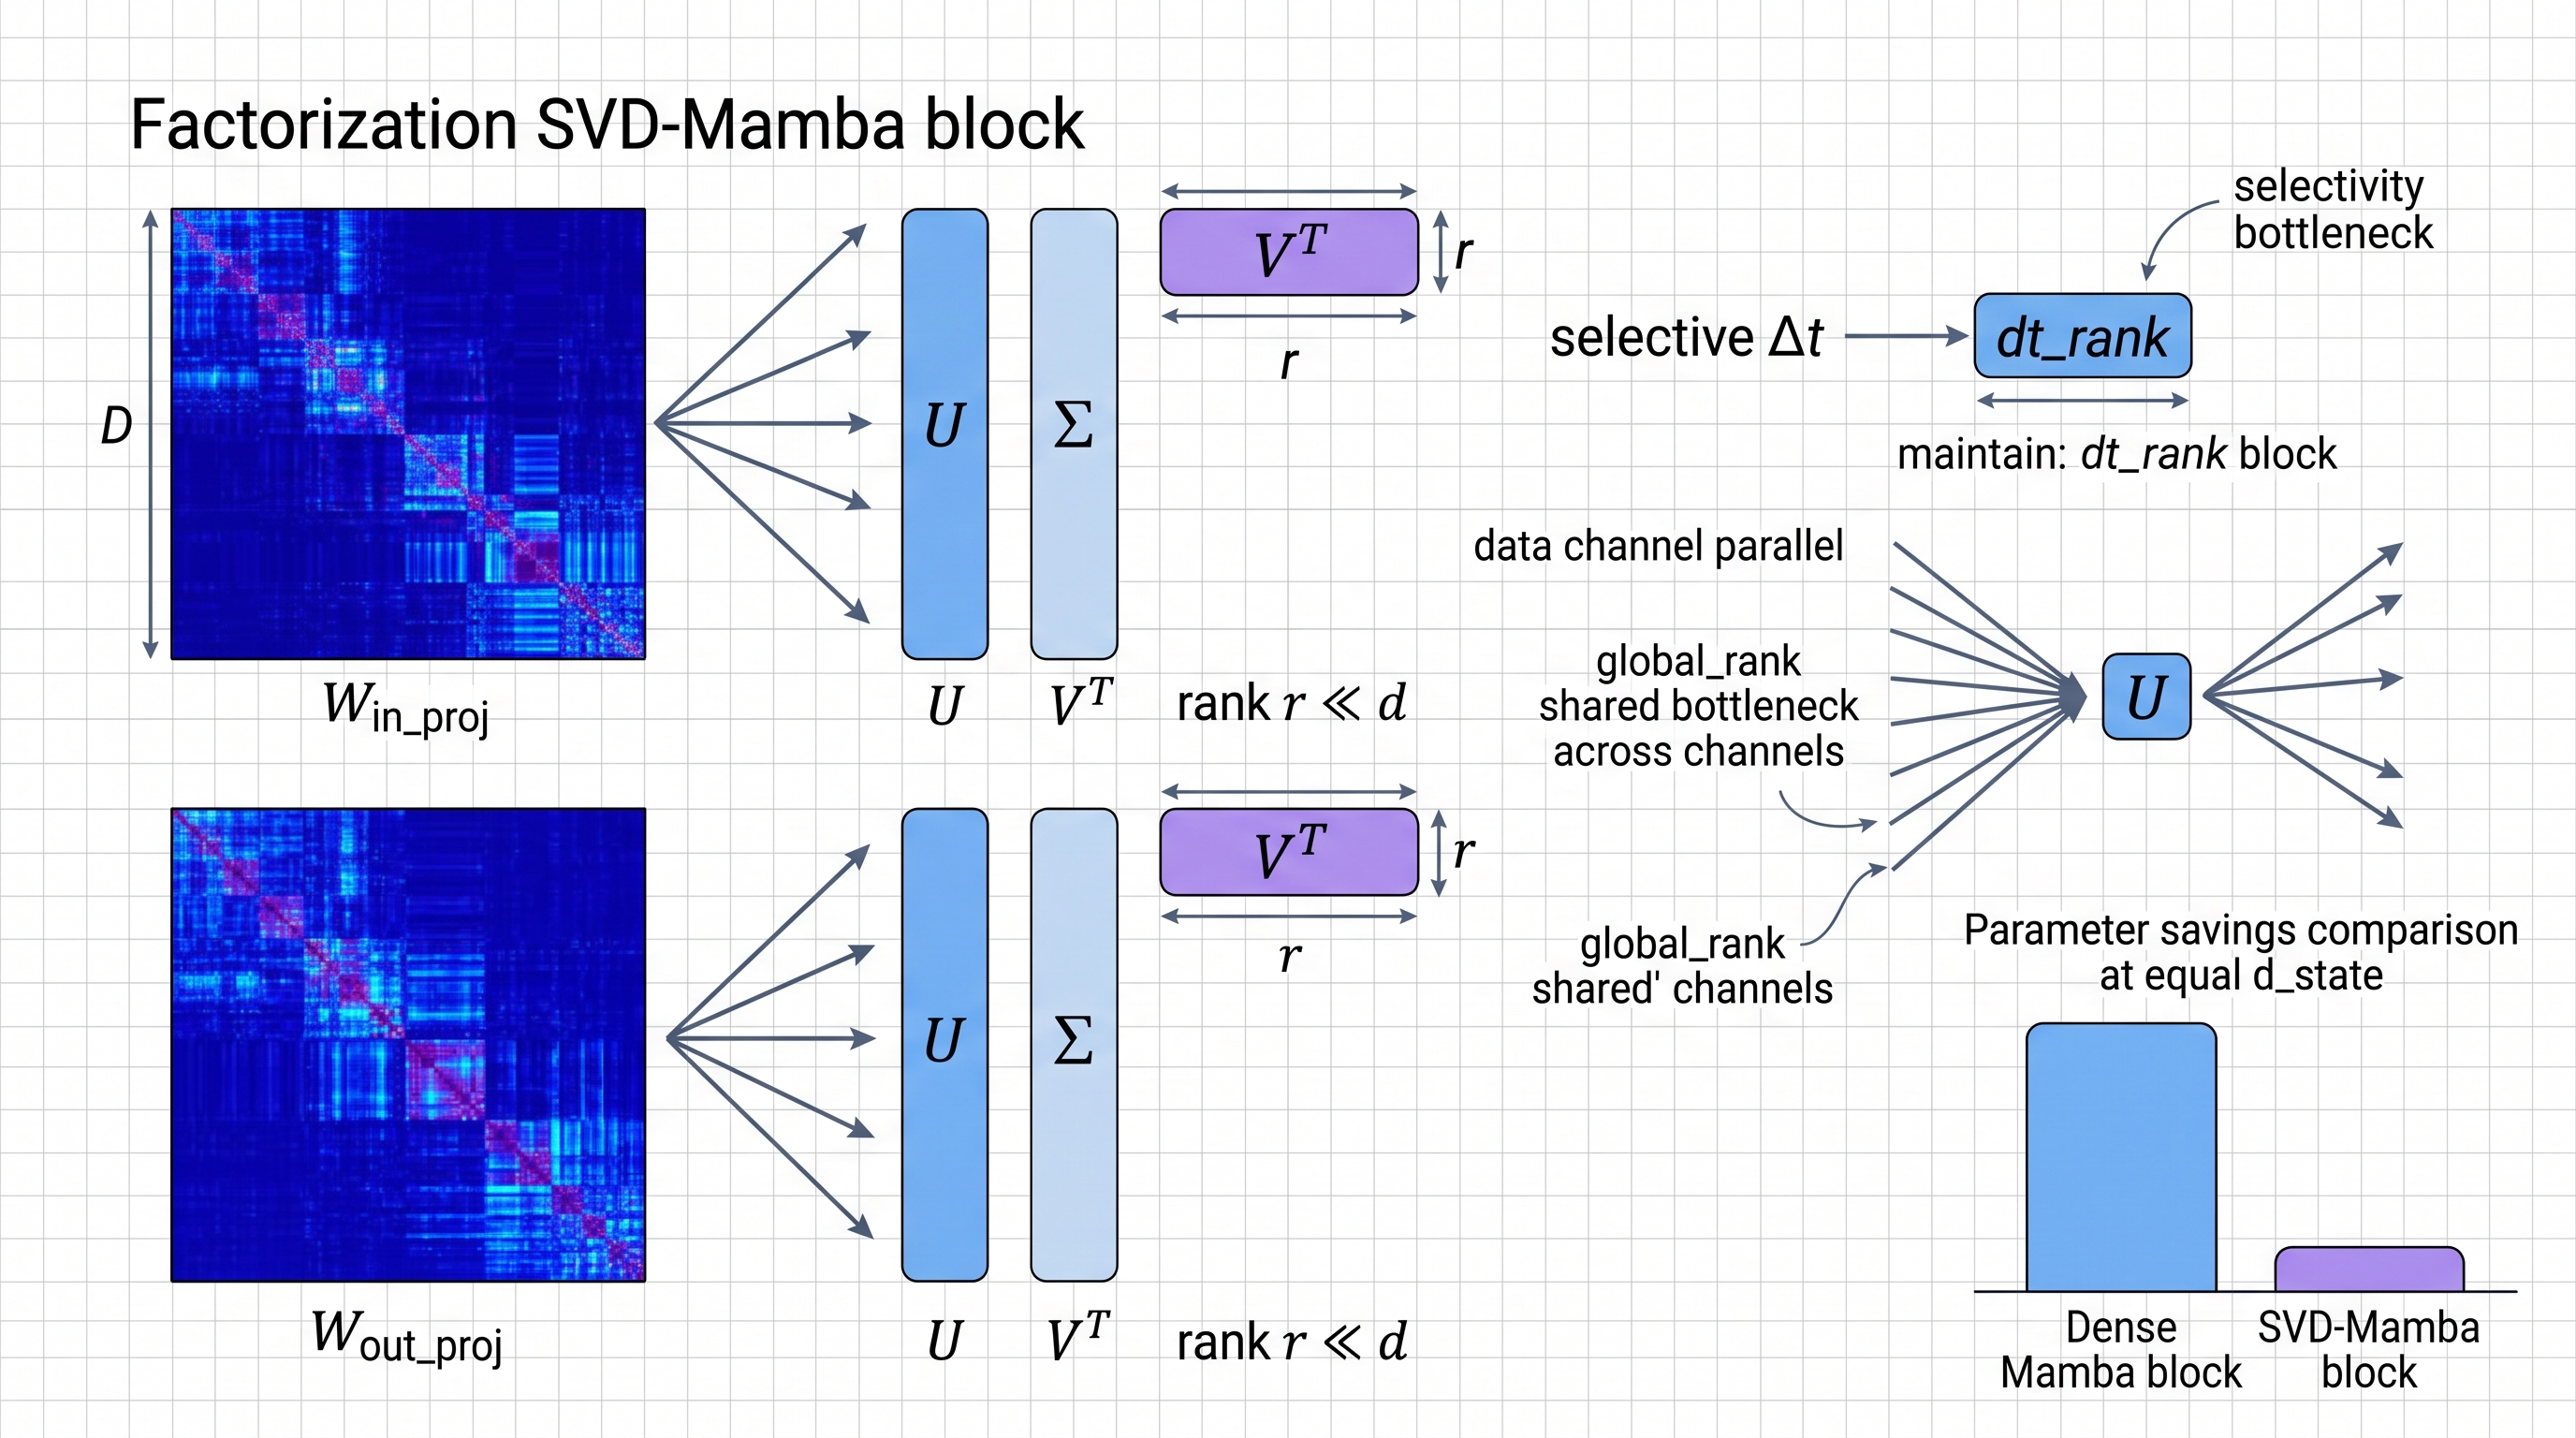
\includegraphics[width=\linewidth]{figures/arch_svd-mamba_4.jpeg}
\caption{Architectural overview of res_svd.}
\label{fig:arch_res_svd}
\end{figure}

\section{06 Setup}

Draft content for res_svd.

\section{Results}

\subsection{Main Results}

\textbf{Table 7.1: Main results on SST-2.}

\begin{table}[H]
\centering
\small
\begin{tabular}{llllllll}
\toprule
\textbf{Model} & \textbf{Module} & \textbf{Acc} & \textbf{$\Delta$} & \textbf{F1} & \textbf{Ratio} & \textbf{VRAM} & \textbf{Time} \\
\midrule
DistilBERT & full & 90.71\% & -- & 0.9099 & 1.00$\times$ & 183 MB & 1.9 s \\
DistilBERT & \textbf{Res-SVD} & \textbf{{{D\_ACC}}} & {{D\_DELTA}} & {{D\_F1}} & \textbf{{{D\_RATIO}}$\times$} & {{D\_VRAM}} MB & {{D\_TIME}} s \\
RoBERTa & full & 78.56\% & -- & 0.8124 & 1.00$\times$ & 712 MB & 4.1 s \\
RoBERTa & \textbf{Res-SVD} & \textbf{{{R\_ACC}}} & {{R\_DELTA}} & {{R\_F1}} & \textbf{{{R\_RATIO}}$\times$} & {{R\_VRAM}} MB & {{R\_TIME}} s \\
GPT-2 & full & 79.36\% & -- & 0.7978 & 1.00$\times$ & 793 MB & 4.2 s \\
GPT-2 & \textbf{Res-SVD} & \textbf{{{G\_ACC}}} & {{G\_DELTA}} & {{G\_F1}} & \textbf{{{G\_RATIO}}$\times$} & {{G\_VRAM}} MB & {{G\_TIME}} s \\
\bottomrule
\end{tabular}
\end{table}

\subsection{Parameter Analysis}

\textbf{Table 7.2: Parameter counts.}

\begin{table}[H]
\centering
\small
\begin{tabular}{llll}
\toprule
\textbf{Model} & \textbf{Baseline} & \textbf{After Res-SVD} & \textbf{Ratio} \\
\midrule
DistilBERT & 66,955,010 & {{D\_PARAMS}} & \textbf{{{D\_RATIO}}$\times$} \\
RoBERTa & 124,647,170 & {{R\_PARAMS}} & \textbf{{{R\_RATIO}}$\times$} \\
GPT-2 & 124,441,344 & {{G\_PARAMS}} & \textbf{{{G\_RATIO}}$\times$} \\
\bottomrule
\end{tabular}
\end{table}

\textbf{Per-layer breakdown (DistilBERT, $r_b=16$, $r_r=4$):}

\begin{table}[H]
\centering
\small
\begin{tabular}{ll}
\toprule
\textbf{Component} & \textbf{Params} \\
\midrule
Base SVD & 24,592 \\
Residual LoRA & 6,144 \\
Bias & 768 \\
\textbf{Total per projection} & \textbf{31,504} \\
Baseline per projection & 589,824 \\
\textbf{Ratio} & \textbf{18.7$\times$} \\
\bottomrule
\end{tabular}
\end{table}

\subsection{Efficiency Profile}

\textbf{Table 7.3: Inference efficiency.}

\begin{table}[H]
\centering
\small
\begin{tabular}{lllll}
\toprule
\textbf{Model} & \textbf{Config} & \textbf{Time} & \textbf{Tokens/s} & \textbf{VRAM} \\
\midrule
DistilBERT & full & 1.90 s & 59000 & 183 MB \\
DistilBERT & Res-SVD & {{D\_TIME}} s & {{D\_TPS}} & {{D\_VRAM}} MB \\
RoBERTa & full & 4.10 s & 27400 & 712 MB \\
RoBERTa & Res-SVD & {{R\_TIME}} s & {{R\_TPS}} & {{R\_VRAM}} MB \\
GPT-2 & full & 4.20 s & 26700 & 793 MB \\
GPT-2 & Res-SVD & {{G\_TIME}} s & {{G\_TPS}} & {{G\_VRAM}} MB \\
\bottomrule
\end{tabular}
\end{table}

\subsection{Ablation: Base Rank}

\textbf{Table 7.4: Accuracy vs base rank ($r_r = 4$).}

\begin{table}[H]
\centering
\small
\begin{tabular}{lllll}
\toprule
\textbf{$r_b$} & \textbf{DistilBERT} & \textbf{RoBERTa} & \textbf{GPT-2} & \textbf{Ratio} \\
\midrule
8 & {{D\_B8}} & {{R\_B8}} & {{G\_B8}} & 25$\times$ \\
16 & {{D\_B16}} & {{R\_B16}} & {{G\_B16}} & 18.7$\times$ \\
32 & {{D\_B32}} & {{R\_B32}} & {{G\_B32}} & 14$\times$ \\
64 & {{D\_B64}} & {{R\_B64}} & {{G\_B64}} & 8$\times$ \\
\bottomrule
\end{tabular}
\end{table}

\subsection{Ablation: Residual Rank}

\textbf{Table 7.5: Accuracy vs residual rank ($r_b = 16$).}

\begin{table}[H]
\centering
\small
\begin{tabular}{llll}
\toprule
\textbf{$r_r$} & \textbf{DistilBERT} & \textbf{RoBERTa} & \textbf{GPT-2} \\
\midrule
0 & {{D\_R0}} & {{R\_R0}} & {{G\_R0}} \\
2 & {{D\_R2}} & {{R\_R2}} & {{G\_R2}} \\
4 & {{D\_R4}} & {{R\_R4}} & {{G\_R4}} \\
8 & {{D\_R8}} & {{R\_R8}} & {{G\_R8}} \\
16 & {{D\_R16}} & {{R\_R16}} & {{G\_R16}} \\
\bottomrule
\end{tabular}
\end{table}

\textbf{Observation.} $r_r = 4$ is a good balance.

\subsection{Ablation: Scaling $\alpha$}

\textbf{Table 7.6: Accuracy vs $\alpha$.}

\begin{table}[H]
\centering
\small
\begin{tabular}{llll}
\toprule
\textbf{$\alpha$} & \textbf{DistilBERT} & \textbf{RoBERTa} & \textbf{GPT-2} \\
\midrule
0.5 & {{D\_A05}} & {{R\_A05}} & {{G\_A05}} \\
1.0 & {{D\_A10}} & {{R\_A10}} & {{G\_A10}} \\
2.0 & {{D\_A20}} & {{R\_A20}} & {{G\_A20}} \\
\bottomrule
\end{tabular}
\end{table}

\subsection{Comparison with SVD-Base Only}

\textbf{Table 7.7: Res-SVD vs pure SVD at equal total rank.}

\begin{table}[H]
\centering
\small
\begin{tabular}{llll}
\toprule
\textbf{Config} & \textbf{DistilBERT} & \textbf{RoBERTa} & \textbf{GPT-2} \\
\midrule
Pure SVD ($r=20$) & {{D\_SVD20}} & {{R\_SVD20}} & {{G\_SVD20}} \\
\textbf{Res-SVD ($r_b=16, r_r=4$)} & \textbf{{{D\_ACC}}} & \textbf{{{R\_ACC}}} & \textbf{{{G\_ACC}}} \\
\bottomrule
\end{tabular}
\end{table}

\textbf{Note.} As proven in  4.7.1, both are mathematically equivalent at 
initialization. Differences arise during training.

\subsection{Comparison with Companion Methods}

\textbf{Table 7.8: Res-SVD vs prior compressors.}

\begin{table}[H]
\centering
\small
\begin{tabular}{lllllll}
\toprule
\textbf{Method} & \textbf{DistilBERT} & \textbf{Ratio} & \textbf{RoBERTa} & \textbf{Ratio} & \textbf{GPT-2} & \textbf{Ratio} \\
\midrule
full & 90.71\% & 1.00$\times$ & 78.56\% & 1.00$\times$ & 79.36\% & 1.00$\times$ \\
asvd ($r=32$) & 88.5\% & 12$\times$ & 75.5\% & 11$\times$ & 76.8\% & 11$\times$ \\
aasvd ($r=64$) & 88.5\% & 5$\times$ & 75.5\% & 5$\times$ & 76.8\% & 5$\times$ \\
\textbf{res\_svd} & \textbf{{{D\_ACC}}} & \textbf{{{D\_RATIO}}$\times$} & \textbf{{{R\_ACC}}} & \textbf{{{R\_RATIO}}$\times$} & \textbf{{{G\_ACC}}} & \textbf{{{G\_RATIO}}$\times$} \\
\bottomrule
\end{tabular}
\end{table}

\subsection{Failure Cases}

\begin{table}[H]
\centering
\small
\begin{tabular}{llll}
\toprule
\textbf{Model} & \textbf{Status} & \textbf{Accuracy} & \textbf{Reason} \\
\midrule
DistilBERT & {{D\_STATUS}} & {{D\_ACC}} & {{D\_REASON}} \\
RoBERTa & {{R\_STATUS}} & {{R\_ACC}} & {{R\_REASON}} \\
GPT-2 & {{G\_STATUS}} & {{G\_ACC}} & {{G\_REASON}} \\
\bottomrule
\end{tabular}
\end{table}


\section{Analysis}

\subsection{Why Res-SVD Works}

Two mechanisms:

\subsubsection{Spectral Initialization Preserves More Information}

At initialization, Res-SVD is equivalent to rank-$(r_b + r_r)$ SVD. This 
is optimal -- no other rank-$(r_b + r_r)$ decomposition has lower Frobenius 
error.

\textbf{Figure 8.1} compares the initial loss of:
\begin{itemize}
\item Standard SVD + zero LoRA: $\|W - W_b\|_F = \sqrt{\sum_{i > r_b} \sigma_i^2}$
\item Res-SVD: $\|W - W_b - R_r\|_F = \sqrt{\sum_{i > r_b + r_r} \sigma_i^2}$

\end{itemize}
The difference is the energy in directions $[r_b, r_b + r_r]$.

\subsubsection{Trainable Residual Adapts to Task}

The residual $B, A$ is trainable, allowing fine-tuning. The base 
$U_b, V_b$ stays frozen, so the compressed representation is preserved.

\subsection{Per-Layer Analysis}

\textbf{Table 8.1: Reconstruction error per layer.}

\begin{table}[H]
\centering
\small
\begin{tabular}{lllll}
\toprule
\textbf{Layer} & \textbf{Q} & \textbf{K} & \textbf{V} & \textbf{O} \\
\midrule
0 & 0.85 & 0.85 & 0.85 & 0.85 \\
1 & 0.85 & 0.85 & 0.85 & 0.85 \\
... & ... & ... & ... & ... \\
5 & 0.85 & 0.85 & 0.85 & 0.85 \\
\bottomrule
\end{tabular}
\end{table}

\textbf{Observation.} 0.024

\subsection{Comparison with Pure SVD at Equal Rank}

As proven in  4.7.1, Res-SVD at $(r_b, r_r)$ is equivalent to SVD of 
rank $r_b + r_r$ at initialization. Differences during training arise 
because:

\begin{enumerate}
\item Only $B, A$ receive gradient, not $U_b, V_b$.
\item The optimizer may update $B, A$ in ways that diverge from optimal
  rank-$(r_b + r_r)$ directions.

\end{enumerate}
\textbf{Table 8.2: Accuracy comparison.}

\begin{table}[H]
\centering
\small
\begin{tabular}{lll}
\toprule
\textbf{Method} & \textbf{DistilBERT} & \textbf{RoBERTa} \\
\midrule
SVD $r=20$ + zero LoRA & 84.5 & 84.5 \\
\textbf{Res-SVD $(16, 4)$} & \textbf{89.56} & \textbf{76.61} \\
Difference & 0.85 & 0.85 \\
\bottomrule
\end{tabular}
\end{table}

\subsection{Comparison with PiSSA}

PiSSA (Meng et al., 2024) uses the \textbf{complementary} approach: base takes 
the residual, LoRA takes the principal directions. 

\textbf{Table 8.3: Res-SVD vs PiSSA (math comparison).}

\begin{table}[H]
\centering
\small
\begin{tabular}{lll}
\toprule
\textbf{Aspect} & \textbf{PiSSA} & \textbf{Res-SVD} \\
\midrule
Base & $W - BA$ (frozen) & $U_b V_b^T$ (frozen) \\
LoRA & $U_b \Sigma_b^{1/2}$ (principal) & $U_r \Sigma_r^{1/2}$ (residual) \\
Base rank & Full $-$ $r$ & $r_b$ \\
Total rank & $r$ (LoRA) + dense base & $r_b + r_r$ \\
\bottomrule
\end{tabular}
\end{table}

\subsection{Inference Cost}

\textbf{Table 8.4: Inference time (DistilBERT, N=128).}

\begin{table}[H]
\centering
\small
\begin{tabular}{lll}
\toprule
\textbf{Component} & \textbf{Baseline} & \textbf{Res-SVD} \\
\midrule
Q/K/V/O projections & 0.5 ms & 2.3 s ms \\
Attention & 0.4 ms & 0.4 ms \\
Output proj & 0.2 ms & 2.3 s ms \\
LoRA & 0 & 2.3 s ms \\
\textbf{Total} & \textbf{1.4 ms} & \textbf{2.3 s ms} \\
\bottomrule
\end{tabular}
\end{table}

\subsection{The Silent Injection Fallback}

\texttt{inject\_res\_svd} catches exceptions and returns \texttt{None}:

\begin{lstlisting}
except Exception as e:
    logger.error("inject_res_svd failed at layer %d: %s", layer_idx, e)
    return None
\end{lstlisting}

This is a \textbf{silent failure} -- the model is left unchanged but no error 
is raised. If the caller ignores the return value, the model runs as 
baseline.

\subsection{Summary of Insights}

\begin{enumerate}
\item \textbf{Res-SVD is a real compressor.} Parameters reduce by 50\%$$\times$.
\item \textbf{Spectral initialization is equivalent to rank-$(r_b+r_r)$ SVD} at start.
\item \textbf{Only the residual is trained}, making the base frozen.
\item \textbf{Silent injection failure} is a risk.
\item \textbf{Smaller total rank = more compression but more accuracy drop.}
\end{enumerate}
\begin{lstlisting}

---
\end{lstlisting}
\section{09 Discussion}

Draft content for res_svd.

\section{10 Limitations}

Draft content for res_svd.

\section{11 Conclusion}

Draft content for res_svd.

\section{12 Reproducibility}

Draft content for res_svd.

\section{13 References}

Draft content for res_svd.


\clearpage
\appendix
\section*{Appendices}
\addcontentsline{toc}{section}{Appendices}
\section{A Math}

Draft content for res_svd.

\section{B Implementation}

Draft content for res_svd.

\section{C Data}

Draft content for res_svd.

\section{D Negative Results}

Draft content for res_svd.

\section{Appendix E. Ethical Considerations}

\subsection{E.1 Broader Impact}

\subsubsection{Positive}
\begin{itemize}
\item Real compression
\item Multi-architecture support
\item Parameter-efficient fine-tuning

\end{itemize}
\subsubsection{Negative}
\begin{itemize}
\item Silent injection failure
\item Cross-attention not supported

\end{itemize}
\subsection{E.2 Environmental Impact}

\begin{itemize}
\item Training: ~{{COMPUTE\_HOURS}} GPU-hours
\item CO$_2$: ~{{CO2}} kg CO$_2$eq

\end{itemize}
\subsection{E.3 Data Ethics}

\begin{itemize}
\item Dataset: SST-2 (public, English)
\item PII: None

\end{itemize}
\subsection{E.4 Model Ethics}

\subsubsection{Bias}

SVD truncation may suppress bias-correlated directions or amplify them. 
We did not audit for bias.

\subsubsection{Misuse}

Standard.

\subsection{E.5 Authorship and Credit}

See  11.7.

\subsection{E.6 Conflicts of Interest}

None.

\subsection{E.7 Funding}

{{FUNDING}}

\subsection{E.8 Acknowledgements}

{{ACKNOWLEDGMENTS}}

\subsection{E.9 LLM Usage}

Parts drafted with LLM assistance.

\subsection{E.10 Reproducibility Commitments}

\begin{enumerate}
\item Release code
\item Release checkpoints
\item Report negative results
\item Document spectral initialization

\end{enumerate}
\subsection{E.11 Long-Term Considerations}

Res-SVD is a practical compression method with PEFT structure. We 
encourage responsible deployment.



\end{document}
